\documentclass{report}
\usepackage{graphicx} % Required for inserting images
\usepackage[italian]{babel}
\usepackage{tikz}
\usepackage{hyperref}
\usepackage{amsmath}
\usepackage{xcolor}

\definecolor{darkgreen}{rgb}{0.0, 0.5, 0.0}


\title{Protezione e Integrità degli Accessi}
\date{Parte VI}

\begin{document}

\maketitle

\tableofcontents
\newpage

Garantire la privacy dei dati nel cloud significa garantire anche 
la confidenzialità dell'\textbf{accesso ai dati}:
\begin{itemize}
    \item \textbf{\textit{Access confidentiality:}} garantire confidenziale il fatto 
    che un accesso mira a un determinato dato
    \item \textbf{\textit{Pattern confidentiality:}} confidenzialità del fatto che due accessi 
    mirano allo stesso dato; si vuole proteggere il fatto che un utente abbia fatto la stessa query in due 
    momenti diversi, o che due utenti abbiano fatto la stessa query
\end{itemize}

\chapter{Path ORAM e Ring ORAM}
\section{Path ORAM}

\begin{itemize}
    \item \textbf{Server side}
    \begin{itemize}
        \item Si organizzano i dati in un albero binario 
        \item Ogni nodo contiene è un \textit{bucket} che contiene sia dei dati che dello spazio disponibile 
        \item Ogni nodo foglia $x$ rappresenta un cammino unico $P(x)$ da $x$ alla $root$
    \end{itemize}
    \item \textbf{Client side}
    \begin{itemize}
        \item Si tiene una piccola cache chiamata \textit{stash}
        \item Tiene una \textit{position map:} $x = position[a]$
        
        $\rightarrow$ il blocco $a$ è in qualche \textit{bucket} nel path $P(x)$
        per raggiungere $x$
        \item Ogni volta che viene letto qualcosa i blocchi vengono spostati
    \end{itemize}
\end{itemize}

In ogni momento (\textit{main invariants}):
\begin{itemize}
    \item ciascun blocco è mappato ad un cammino radice-foglia 
    \item quando devo riposizionare un blocco dopo averlo letto, non lo faccio subito 
    (altrimenti vedi dove l'ho messo); vengono tenuti nella memoria locale e poi 
    vengono riallocati durante una nuova lettura 
\end{itemize}
\newpage
\subsubsection{Esempio}
\begin{figure}[ht]
    \centering
    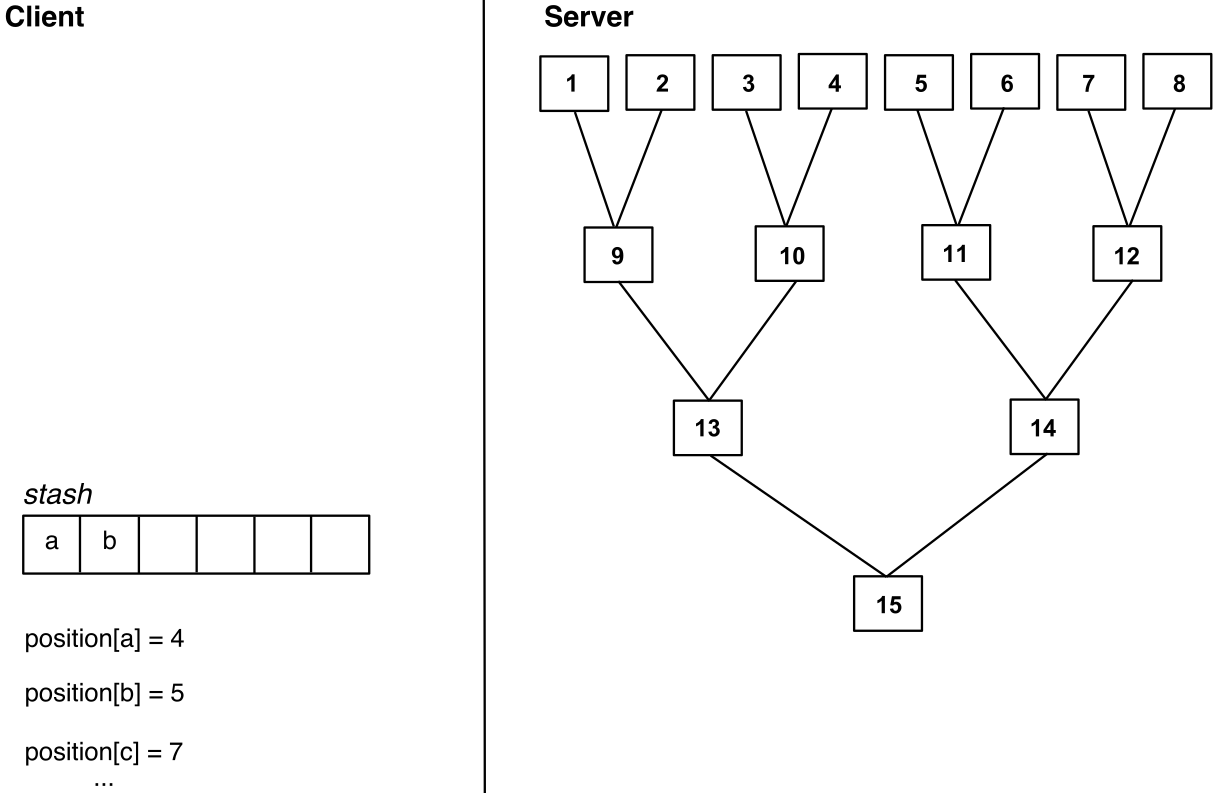
\includegraphics[width=0.8\linewidth]{images/path-oram.png}
\end{figure}

\begin{itemize}
    \item in \textit{stash} abbiamo gli elementi che ancora dobbiamo mettere a posto ($a$ e $b$)
    \item sotto abbiamo la \textit{position map}:
    \begin{itemize}
        \item dobbiamo mettere $a$ in un cammino verso 4
        \item dobbiamo mettere $b$ in un cammino verso 5
        \item sappiamo che $c$ si trova in un cammino verso 7
    \end{itemize}

\end{itemize}

\begin{figure}[ht]
    \centering
    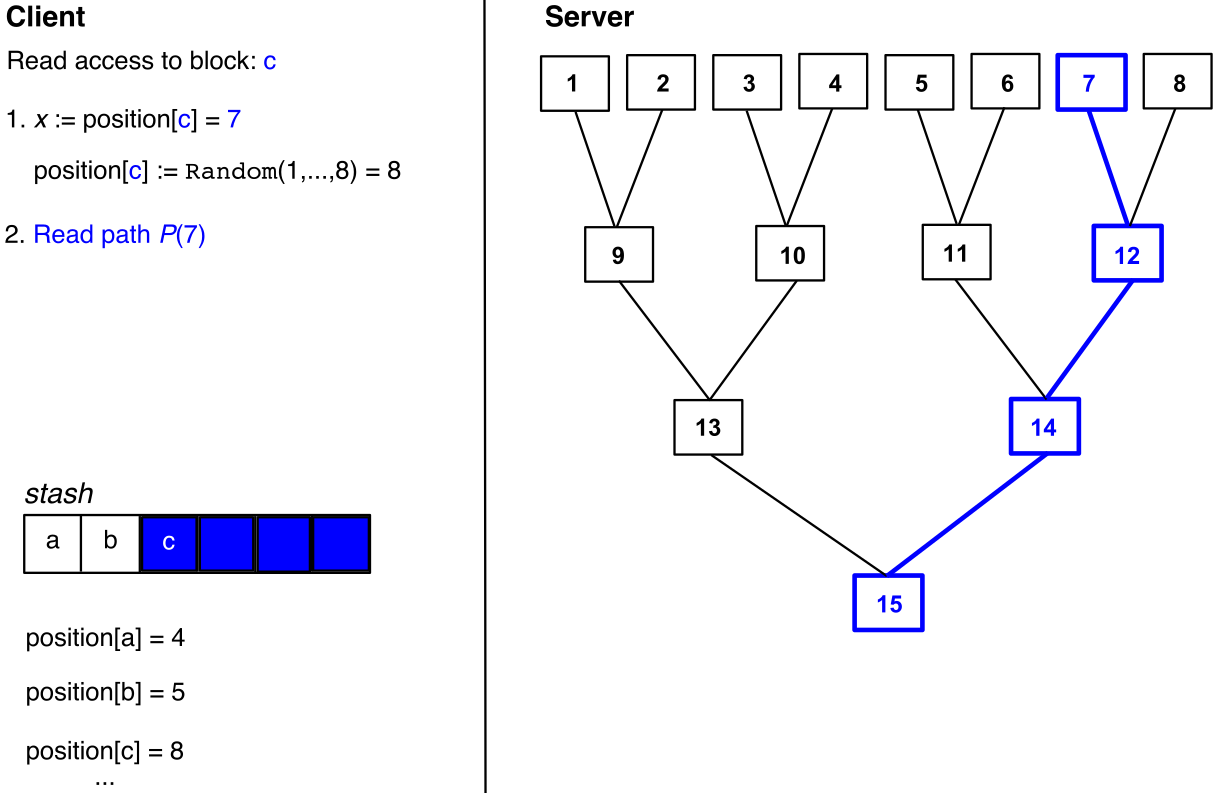
\includegraphics[width=0.8\linewidth]{images/path-oram2.png}
\end{figure}

\begin{itemize}
    \item Leggiamo $c$; dato che sappiamo che dovremo cambiare posto, calcoliamo 
    anche la sua nuova posizione
    \item aggiorniamo la mappa
\end{itemize}

\begin{figure}[ht]
    \centering
    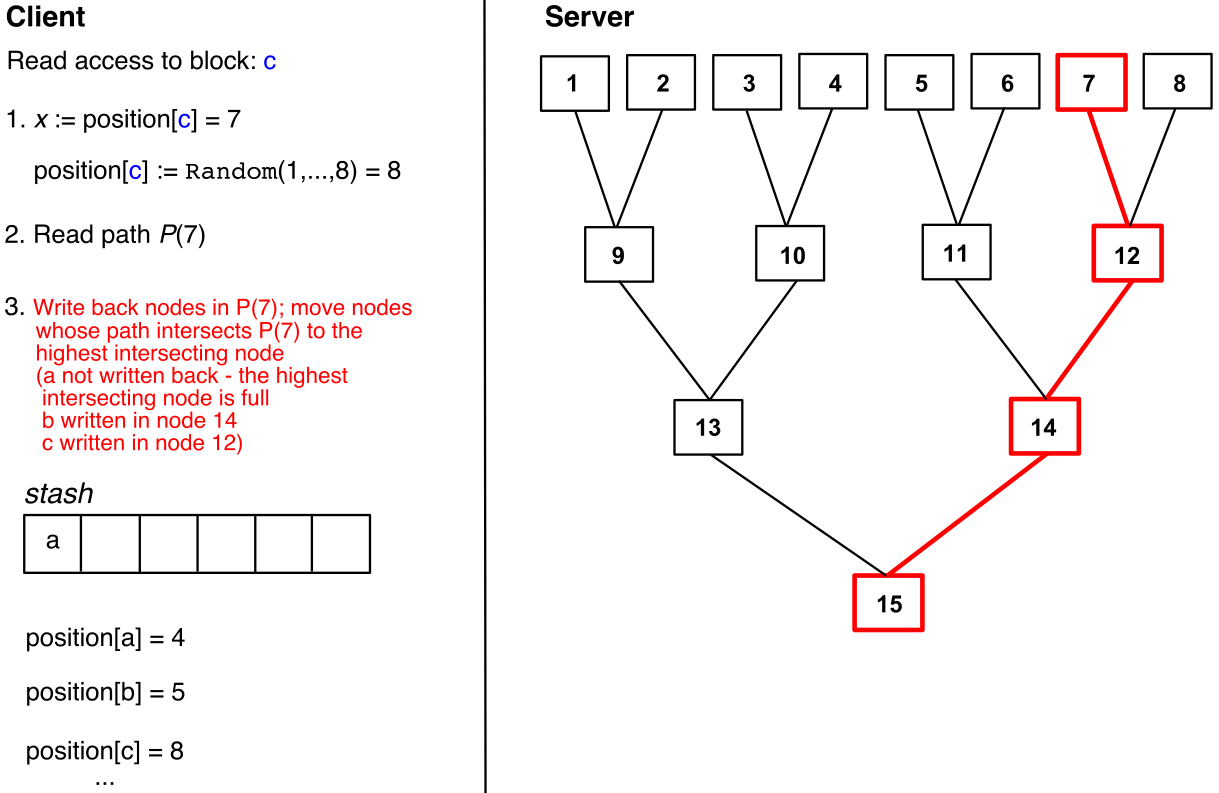
\includegraphics[width=0.8\linewidth]{images/path-oram3.png}
\end{figure}

\begin{itemize}
    \item intanto che percorriamo il cammino $P(7)$ per leggere $c$, ci portiamo 
    tutto quello che possiamo riposizionare dallo \textit{stash}

    $\rightarrow$ io faccio sempre tutto il cammino fino alla foglia, anche perché se mi fermassi prima 
    ti starei spifferando dove ho trovato il blocco
    \item $b$ viene scritto nel nodo 14; $c$ viene scritto nel nodo 12
\end{itemize}

\section{Ring ORAM}
È una variante del Path ORAM; ha la stessa struttura server-side del 
Path ORAM con qualche piccola modifica per la gestione.

\noindent La differenza principale sta nel fatto che non si va 
a rimappare e riscrevere le cose ad ogni accesso, ma viene fatto 
\textit{ogni tanto}.

\section{Vantaggi e Svantaggi}
\begin{itemize}
    \item \textcolor{darkgreen}{\textbf{+}} performance migliorate
    \item \textcolor{red}{\textbf{-}} query di range non supportate
    \item \textcolor{red}{\textbf{-}} accessi da client multipli non supportati 
    \item \textcolor{red}{\textbf{-}} vulnerabile a \textit{failures} del client
\end{itemize}

\chapter{Shuffle Index}
\section{Struttura Dati}
Si utilizza un $B_+$-tree (usati per rispondere anche a query di range):
\begin{itemize}
    \item Segue il ragionamento dell'albero di ricerca
    \item Ogni nodo contiene delle chiavi; deve essere pieno almeno per metà
    \item Tra le chiavi ci sono dei cammini che vanno ai nodi figli; ogni cammino mi
    dice il percorso da seguire per arrivare al valore che mi interessa

    $\rightarrow$ se ho le chiavi $2, 5, 9$:
    \begin{itemize}
        \item per un valore $x < 2$ prendo il cammino a sinistra
        \item per un valore $2 \leq x < 5$ prendo il cammino tra 2 e 5
        \item e così via \dots 
    \end{itemize}

    \item i valori stanno solo nelle foglie; le foglie sono tutte allo stesso 
    livello 
\end{itemize}

\subsubsection{Rappresentazione Astratta}

\begin{figure}[ht]
    \centering
    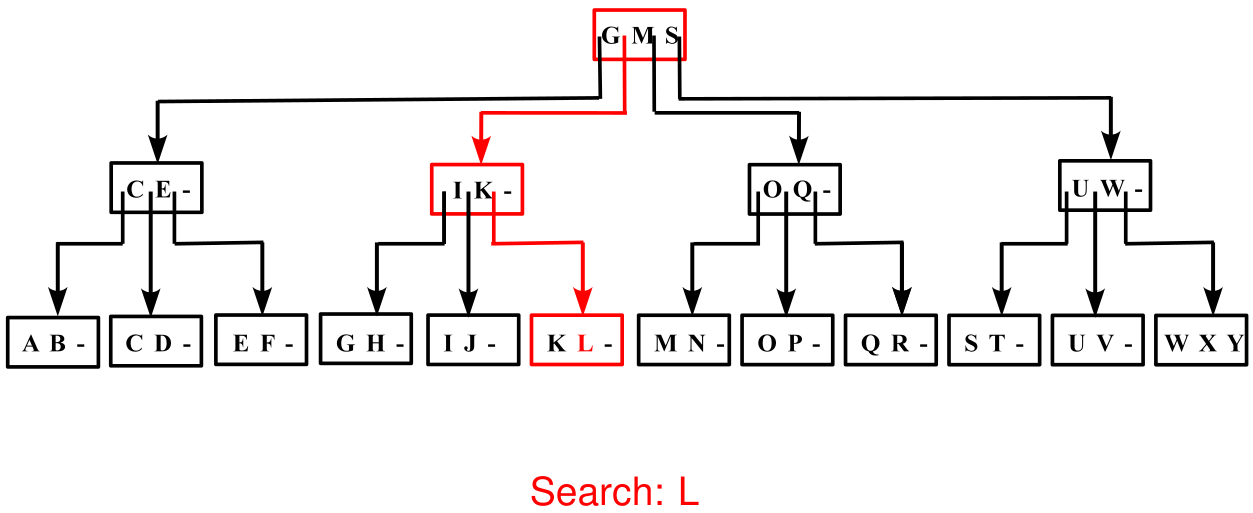
\includegraphics[width=0.91\linewidth]{images/b+-tree.png}
\end{figure}

\subsubsection{Rappresentazione Logica}
I puntatori tra nodi corrispondono, a livello logico, a degli identificatori.

\noindent Avrò un insieme di coppie $\left\langle id, n \right\rangle$ dove:
\begin{itemize}
    \item $id$ identificatore del nodo 
    \item $n$ contenuto del nodo
\end{itemize}

$\rightarrow$ l'ordine degli $id$ non dovrebbe dirmi nulla sull'ordine dei nodi  
nella rappresentazione astratta 

\begin{figure}[ht]
    \centering
    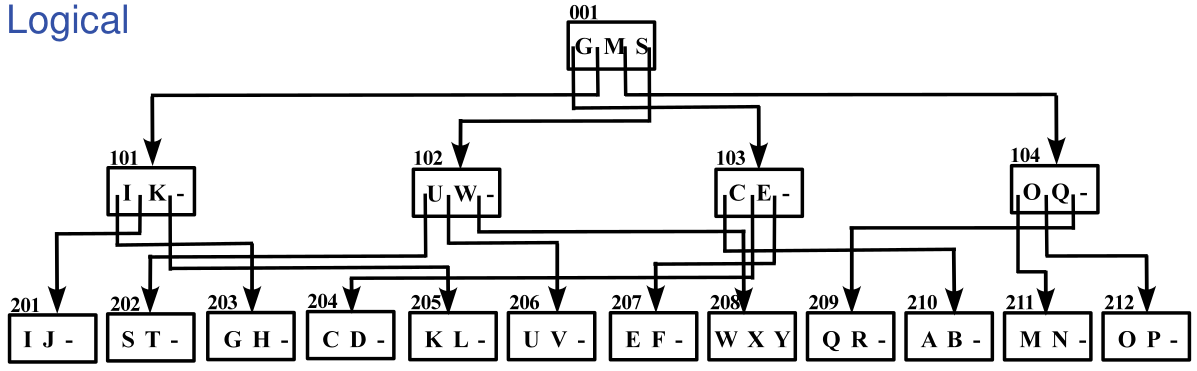
\includegraphics[width=1\linewidth]{images/b+-tree-logical.png}
\end{figure}

\subsubsection{Rappresentazione Fisica}
A livello fisico avrò dei blocchi criptati; ciascuna coppia $\left\langle id, n \right\rangle$ 
corrisponde a una coppia $\left\langle id, b \right\rangle$, dove:
\begin{itemize}
    \item $id$ identificatore 
    \item $b$ è il blocco criptato, costruito come la concatenazione tra:
    \begin{itemize}
        \item cifratura di $n$ con \textit{salt} (il sale serve perché altrimenti anche cambiando posto alle cose, se la criptazione è sempre la stessa tu sei in grado di riconoscerlo)
        \item $id$ del blocco
    \end{itemize}
\end{itemize}

\begin{figure}[ht]
    \centering
    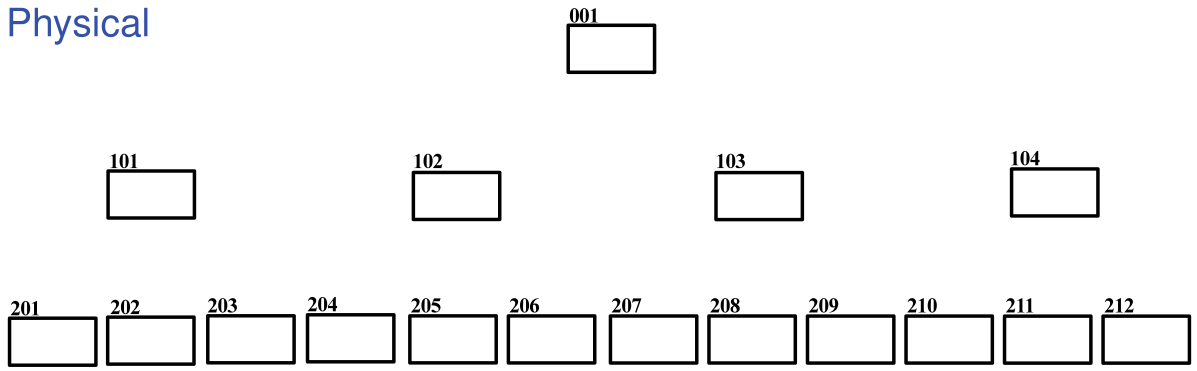
\includegraphics[width=1\linewidth]{images/b+-tree-physical.png}
\end{figure}

\section{Accesso ai dati}
L'accesso ai dati richiede un processo iterativo tra il client e il server;
ad ogni iterazione, il client:
\begin{itemize}
    \item decripta il blocco appena recuperato 
    \item determina il blocco che deve recuperare il server al livello inferiore (verso le foglie)
\end{itemize}

$\rightarrow$ il processo termina quando si raggiunge una foglia

\begin{figure}[ht]
    \centering
    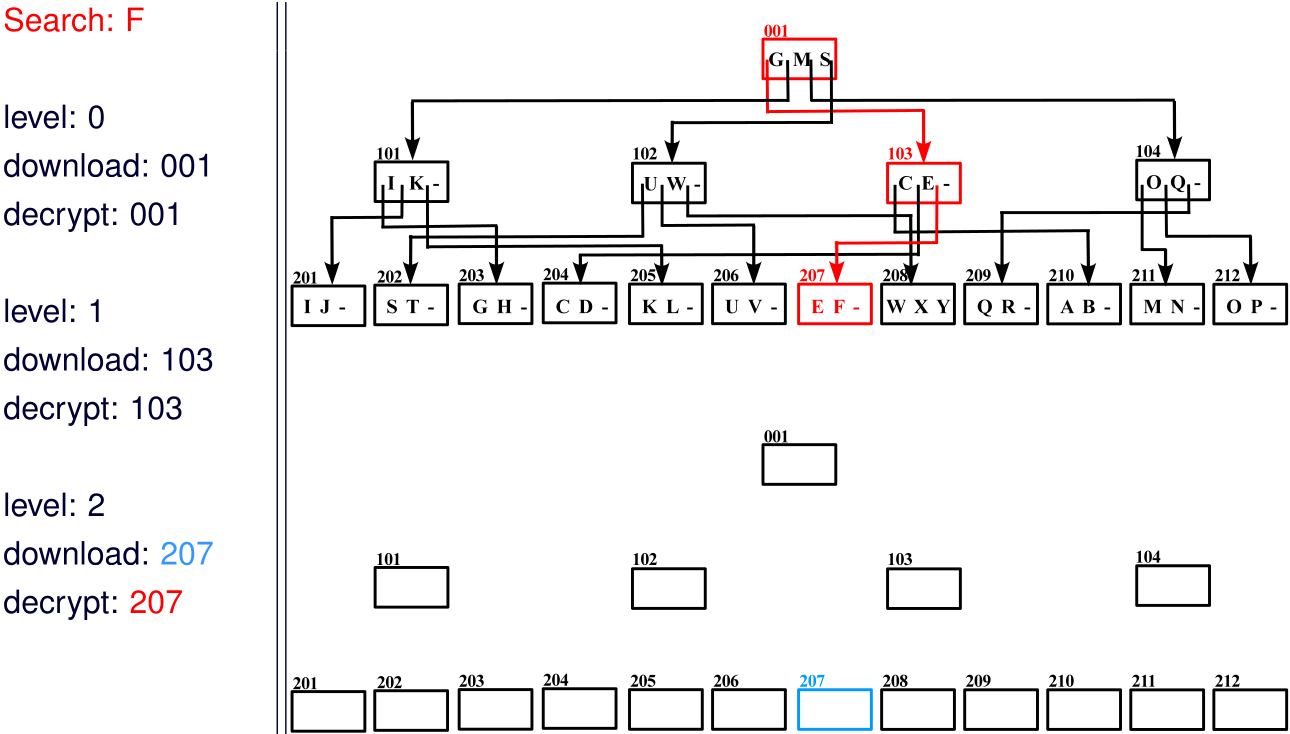
\includegraphics[width=1\linewidth]{images/data-access.png}
\end{figure}

\section{Conoscenza del server}
Il server ottiene una sequenza di blocchi che compongono delle osservazioni:
\begin{itemize}
    \item $o_i = \{ b_{i1}, b_{i2}, \dots, b_{ih} \}$
\end{itemize}

\noindent Il server può inferire facilmente:
\begin{itemize}
    \item il numero $m$ di blocchi e i loro identificatori 
    \item il livello associato ad ogni blocco 
    \item altezza dell'albero
\end{itemize}

\newpage
\subsubsection{La cifratura basta?}
\begin{itemize}
    \item \textcolor{darkgreen}{\textbf{+ protegge}}  
    \begin{itemize}
        \item contenuto dei dati 
        \item contenuto del singolo accesso 
    \end{itemize}
    \item \textcolor{red}{\textbf{- non protegge}}
    \begin{itemize}
        \item \textit{access confidentiality}
        \item \textit{pattern confidentiality}
        
        $\rightarrow$ quando cerco un dato lo trovo sempre nella stessa posizione
    \end{itemize}
\end{itemize}

$\rightarrow$ \textbf{attacchi basati su frequenze possono permettere al server 
di ricostruire i valori in chiaro}

\section{Tecniche di protezione}
Per proteggermi l'obiettivo è \textbf{rompere la corrispondenza tra contenuto e luogo 
in cui è memorizzato }

\noindent Si combinano 3 strategie.

\subsection{\textit{Cover searches}}
\begin{itemize}
    \item Introduce confusione sul target di un accesso, nascondendolo tra un gruppo 
    di altre richieste che fanno da \textit{cover}
    \item Il numero di richieste di cover $num\_cover$ è il parametro di protezione
    \item Le \textit{cover searches} devono:
    \begin{itemize}
        \item fornire \textbf{diversità} tra blocchi 
        \item essere \textbf{indistinguibili} dalla ricerca reale
    \end{itemize}
\end{itemize}

\begin{figure}[ht]
    \centering
    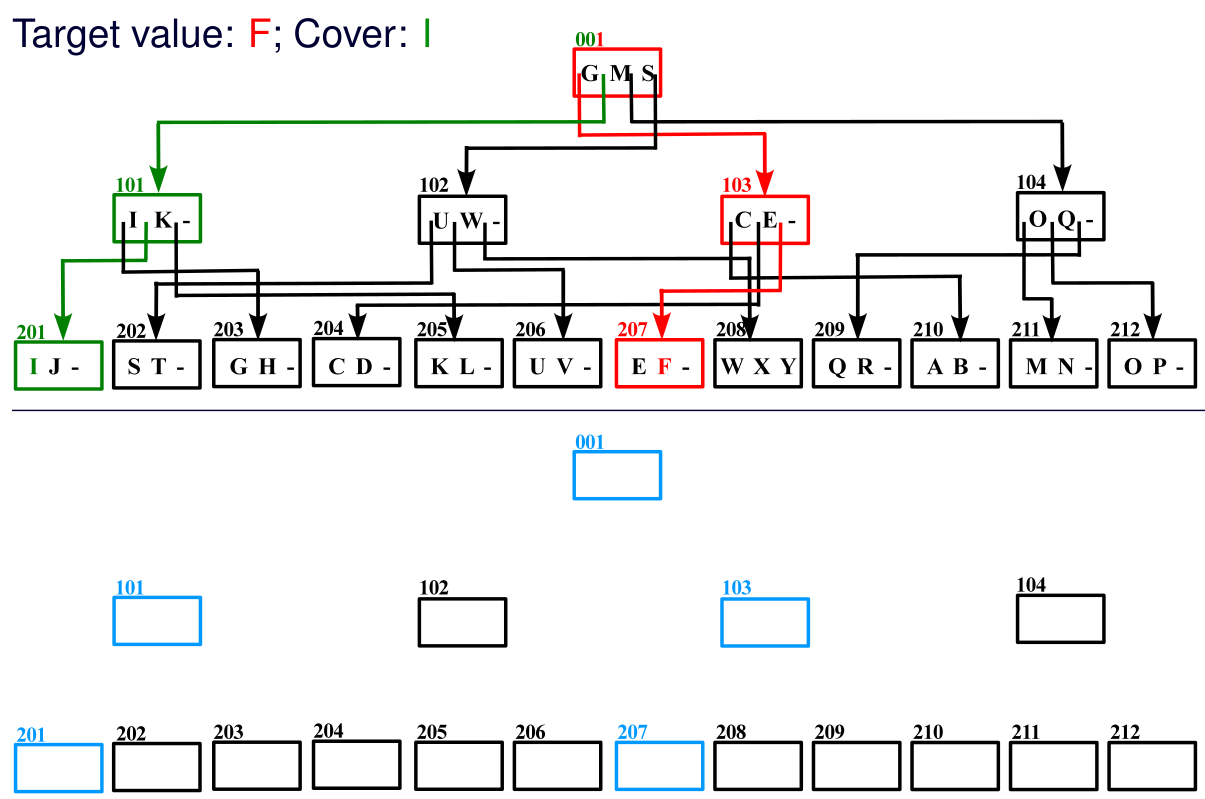
\includegraphics[width=1\linewidth]{images/cover-searches.png}
\end{figure}

\subsubsection{Protezione offerta}
\begin{itemize}
    \item \textcolor{darkgreen}{\textbf{+}} le foglie hanno la stessa probabilità 
    di avere il vero target 
    \item \textcolor{darkgreen}{\textbf{+}} le relazioni tra nodi padre-figlio vengono confuse (\textit{
    il blocco 201 potrebbe essere figlio di 101 o 103})
    \item \textcolor{red}{\textbf{-}} le relazioni padre-figlio possono essere inferite con attacchi di intersezione
\end{itemize}

\subsection{\textit{Cached searches}}
Il client tiene una cache di nodi:
\begin{itemize}
    \item di dimensione $num_cache$, che stabilisce la dimensione per ciascun livello 
    \item se un nodo è presente, allora è presente anche il suo genitore
    \item ogni volta che leggo qualcosa lo metto nella cache 
    \item gestisco la cache con politica \textit{Last Recent Used}
    \item se il target è nella cache, vengono fatte solo delle \textit{cover searches}
\end{itemize}

\subsubsection{Protezione offerta}
\begin{itemize}
    \item \textcolor{darkgreen}{\textbf{+}} protegge da attacchi di intersezione
    \item \textcolor{red}{\textbf{-}} protegge solo finché sto nella dimensione della cache
\end{itemize}

\subsection{\textit{Shuffling}}
\begin{itemize}
    \item Rompe la corrispondenza tra blocchi e nodi, mescolando ogni volta il contenuto in maniera casuale
    \item Ogni volta devo decriptare e re-criptare per poter mescolare
\end{itemize}

\newpage
\section{Analisi della protezione}
\begin{itemize}
    \item con lo \textit{shuffling} rompo la corrispondenza nodo-blocco, riuscendomi a proteggere 
    da attacchi di intersezione
    \item \textbf{\textit{Access confidentiality:}} ogni accesso deve essere diviso tra $num\_cover + 1$ richieste;
    in più lo \textit{shuffling} rompe la corrispondenza nodo-blocco
    \item \textbf{\textit{Pattern confidentiality:}} ci si riesce a proteggere con:
    \begin{itemize}
        \item breve termine con cover e cache 
        \item lungo termine con cover e shuffling
    \end{itemize}
\end{itemize}

\section{Protezione vs Performance}
\begin{itemize}
    \item \textcolor{red}{\textbf{-}} un accesso di lettura implica $num\_cover + num\_cache + 1$ scritture al server 
    \item \textcolor{red}{\textbf{-}} gli accessi concorrenti diventano accessi esclusivi 
    \item \textcolor{darkgreen}{\textbf{+}} migliori performance di Path ORAM 
    \item \textcolor{darkgreen}{\textbf{+}} non ci sono soluzioni che offrono la stessa protezione a performance migliori
\end{itemize}







\end{document}